%%%%%%%%%%%%%%%%%%%%%%%%%%%%%%%%%%%%%%%%%%%%%%%%%%%%%%%%%%%
% --------------------------------------------------------
%  _____           
% |_   _|_ _ _   _ 
%   | |/ _` | | | |
%   | | (_| | |_| |
%   |_|\__,_|\__,_|
%
% LaTeX2e Template
% Version 2.5.0 (01/01/2026)
%
% Author: 
% Guillermo Jimenez (memo.notess1@gmail.com)
% 
% License:
% Creative Commons CC BY 4.0
% --------------------------------------------------------
%%%%%%%%%%%%%%%%%%%%%%%%%%%%%%%%%%%%%%%%%%%%%%%%%%%%%%%%%%%
% --------------------------------------------------------
% Github Repository:
% https://github.com/MemoJimenez/Tau-class
% --------------------------------------------------------
%%%%%%%%%%%%%%%%%%%%%%%%%%%%%%%%%%%%%%%%%%%%%%%%%%%%%%%%%%%

\documentclass[9pt,a4paper,twocolumn,twoside]{tau-class/tau}
\usepackage[english]{babel}

% Spanish babel recomendation
% \usepackage[spanish,es-nodecimaldot,es-noindentfirst]{babel} 

%----------------------------------------------------------
% Title & Authors/Affiliations
%----------------------------------------------------------

\doctype{Assignment Report}
\title{COL780 - AR Tags Analysis}

%----------------------------------------------------------

\author[a,1]{Shahid Khan\thanks{\href{mailto:ee1221163@iitd.ac.in}{ee1221163@iitd.ac.in} (A. One)}}


%----------------------------------------------------------



%----------------------------------------------------------
% Document-, Footer- information
%----------------------------------------------------------

\dates{\today}

% \docinfo{The Document is the report of the assignment 1 of COL780 - Computer Vision course.} 


%----------------------------------------------------------


%----------------------------------------------------------
% ABSTRACT AND KEYWORDS
%----------------------------------------------------------


    % Tau ($\tau$) is a specially designed document class for creating professional and well-structured research articles, technical reports, and academic documentation. Tau enhances the writing experience through intuitive custom environments, multilingual support, and refined typography powered by Fira Sans for headings and distinctive elements, Fira Modo for listings, and STIX2 for body text, providing consistent and professional styling for elements such as tables, figures, equations, code listings, and captions. \textit{New/Updated features will show a (*) in their title.}

%----------------------------------------------------------

%----------------------------------------------------------

\begin{document}
		
    \maketitle 
    \thispagestyle{firststyle}
    
%----------------------------------------------------------

\section{Detection and Identification of AR Tags} 
    video\_link - \href{https://drive.google.com/drive/folders/1yq0wepZofnC9S_1A7GuBsgRKsac3On8C?usp=drive_link}{click\_here}
    \newline
    \textbf{Step 1: Thresholding} — We Convert the input frame to grayscale using weighted RGB combination $(0.299R + 0.587G + 0.114B)$ and apply a fixed threshold value of 200 to create a binary image where white A4 sheets are clearly distinguished from the background.
    
    \textbf{Step 2: ROI Separation} — Use a flood-fill algorithm on a downsampled version (by factor of scale) of the binary image to identify separate white regions (islands/ROI). These are the connected white pixels corresponding to different A4 sheets. The downsampling reduces computational complexity from $O(n \times m)$ to $O((n/8) \times (m/8))$ while maintaining accuracy. Each island represents a potential AR tag location.
    
    \textbf{Step 3: Tag Detection} — Now, for each island, we refine the ROI boundaries by expanding them until no more white pixels are found. Within this refined ROI, we apply fast component labeling to find the largest connected black component that does not touch the border. This component represents the AR tag itself. The boundary pixels of this component are extracted using erosion operations.
    
    \textbf{Step 4: Corner Extraction} — Apply convex hull algorithm to the boundary pixels, followed by Douglas-Peucker polygon approximation with adaptive epsilon values (ranging from 0.01 to 0.08 of perimeter) to find exactly 4 corners. The corners are then sorted counter-clockwise starting from the top-left corner based on angular position relative to the centroid.
    
    \textbf{Step 5: Tag Decoding} — We compute a homography matrix from the detected corners to an $8 \times 8$ canonical grid using SVD-based least squares. The implementation approach was adapted from~\cite{rastogi_artag}. For each cell in the grid, sample multiple points (5$\times$5 sub-samples per cell) and use median voting to determine if the cell is white (1) or black (0). This provides robustness against noise.
    
    \textbf{Step 6: Orientation \& ID Extraction} — Identify the orientation by checking which corner cell contains the white orientation marker at positions $(5,5)$, $(5,2)$, $(2,2)$, or $(2,5)$, corresponding to $0^\circ$, $90^\circ$, $180^\circ$, or $270^\circ$ rotations. Rotate the grid to canonical orientation and decode the 4-bit ID from the inner cells at positions $(3,3)$, $(3,4)$, $(4,4)$, and $(4,3)$ using binary encoding $(8 + 4 + 2 + 1)$.
    
    \textbf{Step 7: ARtag Object Creation} — Return an ARtag object containing the corrected corner coordinates, decoded ID, and orientation information for subsequent processing (3D rendering, superimposition, etc.).


    \begin{figure*}[t]
        \centering
        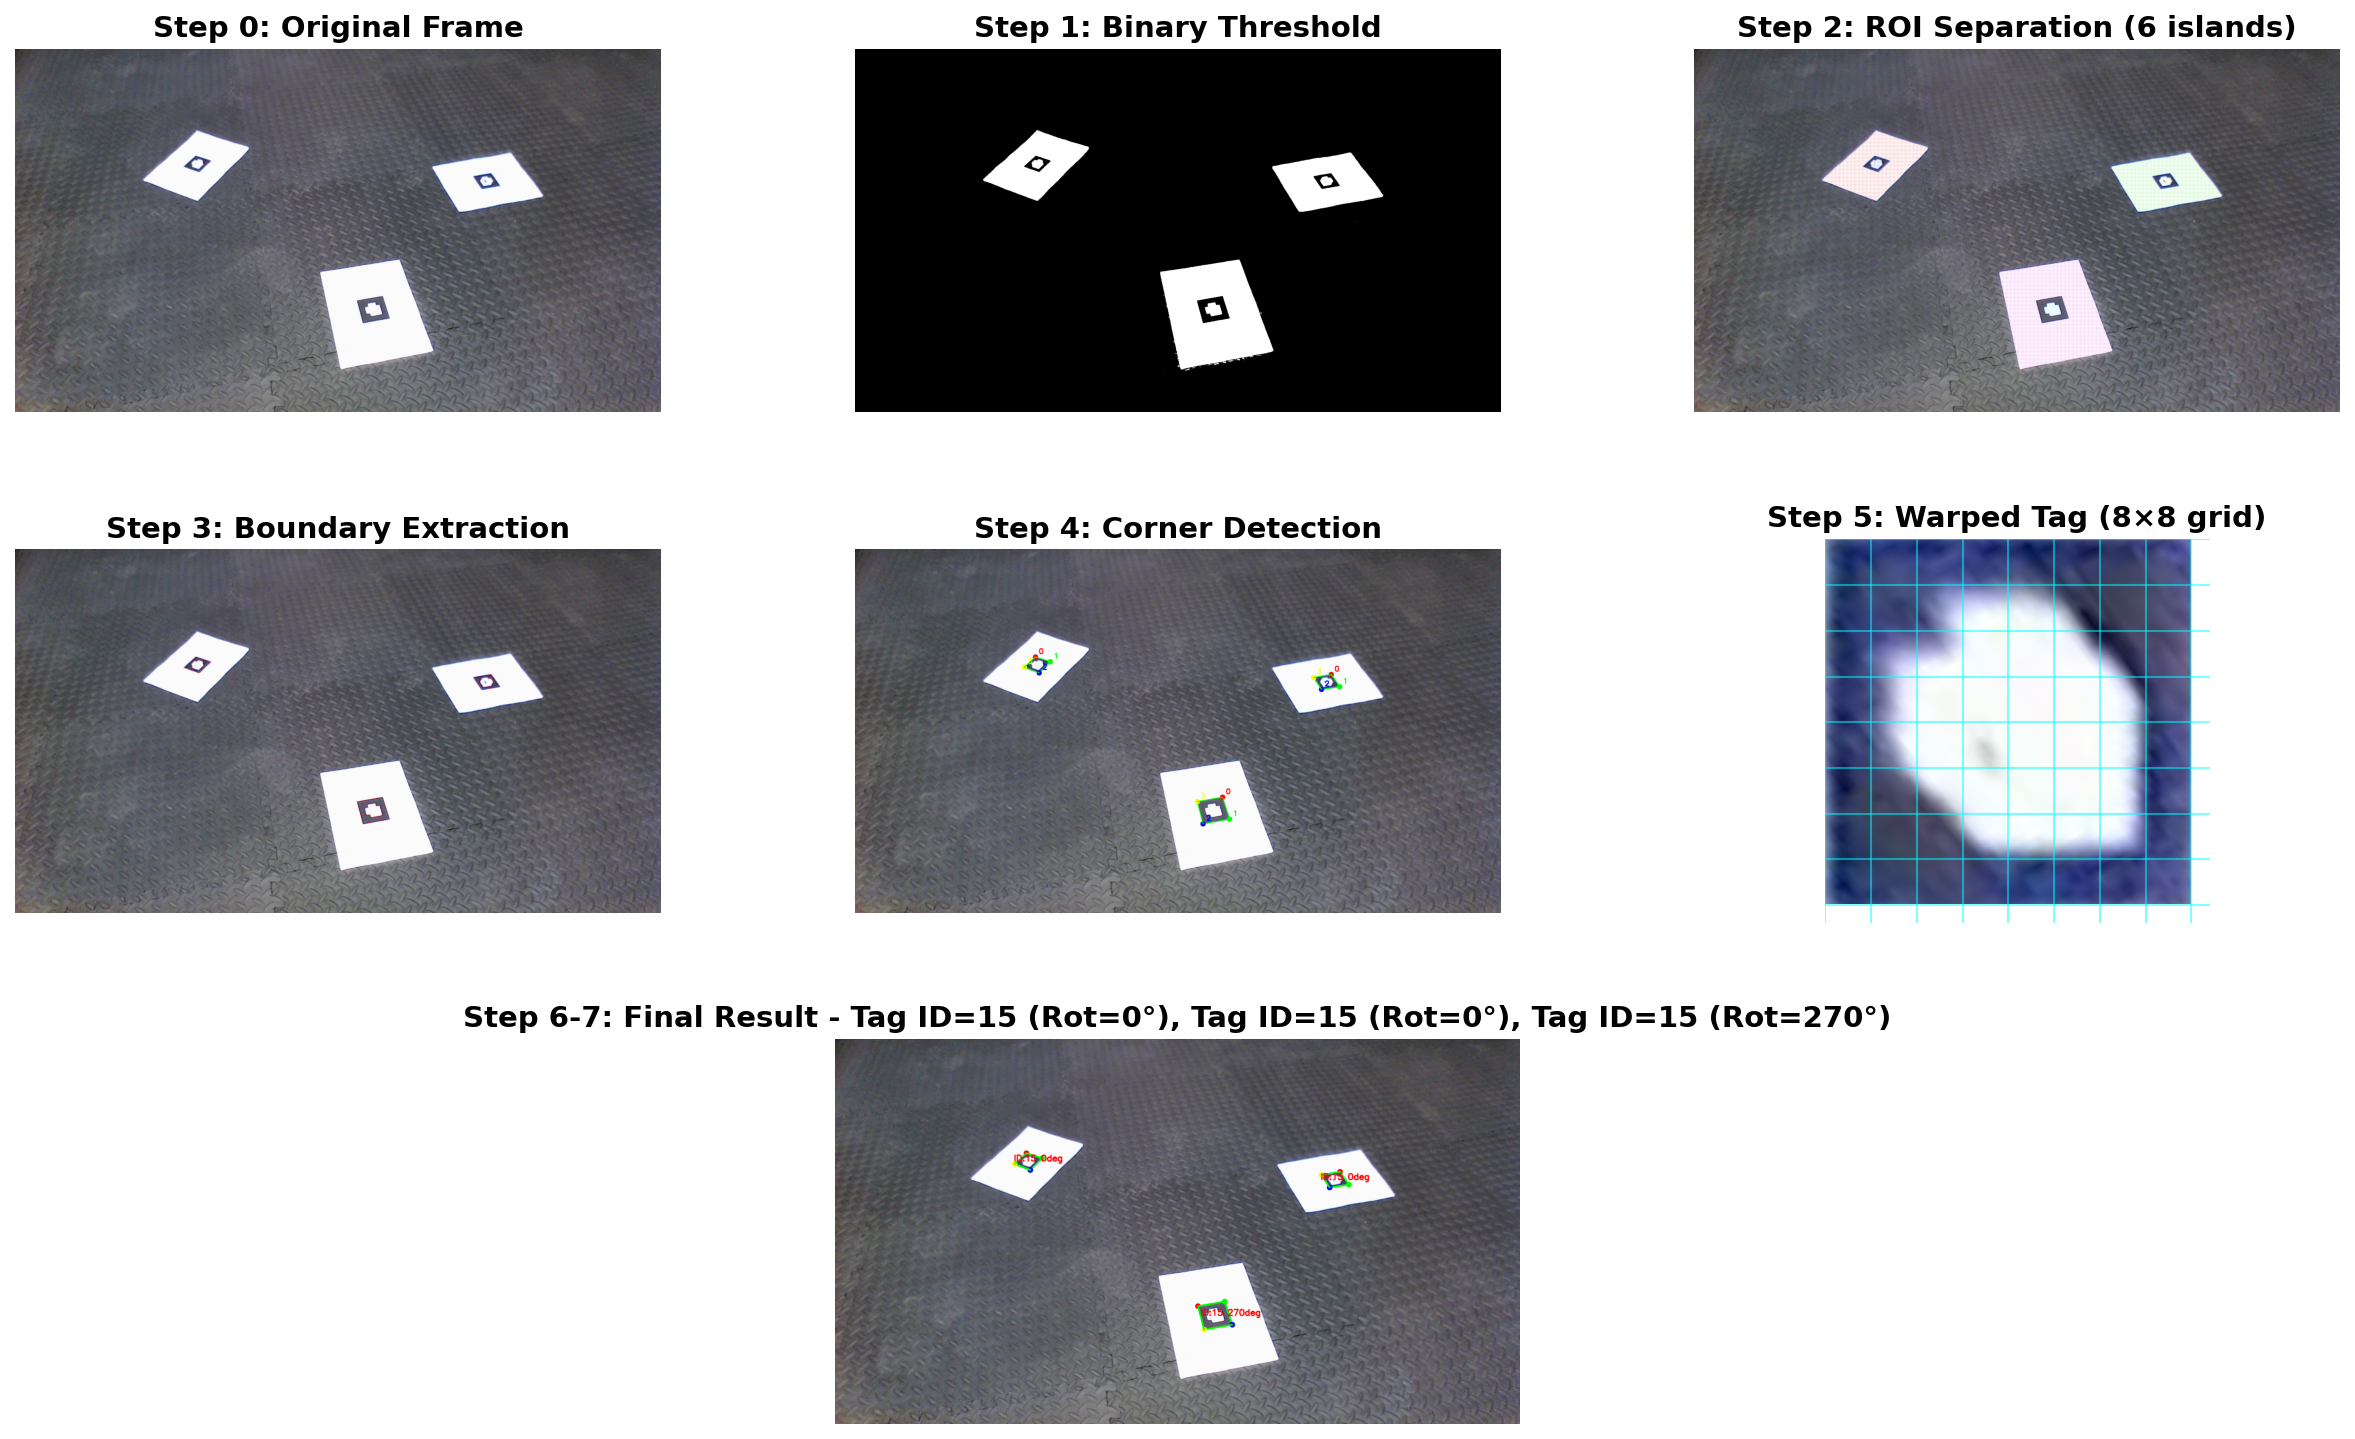
\includegraphics[width=\textwidth]{figures/ar_detection_steps.png}
        \caption{Complete AR tag detection pipeline showing all intermediate steps: (Step 0) Original input frame, (Step 1) Binary thresholding result, (Step 2) ROI separation showing 6 detected islands, (Step 3) Boundary extraction of detected markers, (Step 4) Corner detection with numbered vertices and convex hull, (Step 5) Warped tag showing 8$\times$8 grid overlay, and (Step 6-7) Final result with decoded tag IDs and orientations.}
        \label{fig:ar_detection}
    \end{figure*}

    \figref{fig:ar_detection} illustrates the complete detection pipeline on a sample frame containing multiple AR tags. The algorithm successfully detected 3 tags with ID=15 at various orientations.


\subsection{Challenges Faced:}
    \textbf{Image Size:} The images we were given were of very high resolution (1920 $\times$ 1080), which made processing them computationally expensive. When we were using pure python loops to process the images, our FPS was around 0.2, which was logically not acceptable. To solve this problem, we implemented a number of approaches on top of each other, which eventually let us increase the FPS to around 12. 
    \begin{itemize}
        \item First, we used fast numpy operations to replace the pure python loops, which gave us a significant boost in performance. 
        \item Then, we implemented a downsampling approach to reduce the image size, and hence the complexity. The idea was that once we find the approximate location of the Black Pixels in the downsampled image, we can then go back to the original image, and find the exact location of the black pixels by running a look around algorithm. This approach gave a significant boost in performance, as we were able to reduce the complexity from $O(n \times m)$ to $O((n/8) \times (m/8))$ while still maintaining the accuracy of our detection.
        \item Finally, we used the \textit{numba}~\cite{numba_jit} library to further optimize our code, which actually gave us a significant boost in performance, as we were able to achieve an FPS of around 12, which was a huge improvement from our initial implementation. 
    \end{itemize}

    \textbf{Corner Detection:} One of the main challenges we faced was in the corner detection step. We initially tried using the Harris corner detection algorithm, but it did not work well for our images, as it was not able to accurately detect the corners of the AR tags. We then switched to using the convex hull algorithm followed by the Douglas-Peucker polygon approximation, which gave us much better results. However, we had to experiment with different epsilon values for the Douglas-Peucker algorithm to find the optimal value that would give us exactly 4 corners for each tag.

    \textbf{Noise in the Images in the tag:} If you would lock closely, in the multipleTags.mp4 video, we see that the white portions of two tags have a constantly appearing small black patch, which is corrupting the values of the decoded ID. To solve this problem, we implemented a median voting approach, where we sample multiple points within each cell of the grid, and take the median value to determine if the cell is white or black. This approach proved to be very effective in reducing the impact of noise on our decoding process.
    \newline
    We are still facing some jitter in the marker detection. The jitter mainly comes due to the noise in the detected corners, which we have not able to eliminate completely. This mainly arrives due to the inherent blurring of black and white pixels in the tag, due to which the orientation detection is not always accurate. Also, the Kalman filter make sure there is no flickering, and there is smooth movement of the markers.

\section{2D Augmented Reality}
    video\_link - \href{https://drive.google.com/drive/folders/1bwCFEDMHWHSVKO8GLuNlM5NxsSlA9aG5?usp=sharing}{click\_here}
    \newline
    Once we have detected AR tags and their corners, we can overlay arbitrary 2D images onto the tags to create an augmented reality effect. We try to make this implementation smooth and jitter free by applying Kalman filtering techniques.

    \subsection{Image Overlay Pipeline}

    \textbf{Step 1: Template Loading} — Load the template image that will be overlaid onto detected AR tags. 
    \textbf{Step 2: Tag Detection} — We apply the detection pipeline from Section 1 to identify AR tags in the current frame, obtaining their corner coordinates.

    \textbf{Step 3: Kalman Filtering} — Apply Kalman filtering to smooth the corner trajectories over time. 

    \textbf{Step 4: Homography Computation} — For each detected tag, compute the homography matrix $H$ that maps the template image corners to the smoothed tag corners:
    \begin{equation}
        H: \begin{bmatrix} 0 & 0 \\ w_t & 0 \\ w_t & h_t \\ 0 & h_t \end{bmatrix} \rightarrow \begin{bmatrix} c_0 \\ c_1 \\ c_2 \\ c_3 \end{bmatrix}
    \end{equation}
    where $(w_t, h_t)$ are the template dimensions and $c_i$ are the tracked corner positions.

    \textbf{Step 5: Perspective Warping} — Warp the template image using the computed homography to match the geometric perspective of the detected tag:
    \begin{equation}
        I_{warped}(x, y) = I_{template}(H^{-1}(x, y))
    \end{equation}

    \textbf{Step 6: Mask Generation} — Create a binary mask by warping a white image of the same size as the template. This mask defines the region where the overlay should be applied.

    \textbf{Step 7: Image Composition} — Blend the warped template with the original frame using the mask~\cite{opencv_warp}:
    \begin{equation}
        I_{output}(x, y) = \begin{cases}
            I_{warped}(x, y) & \text{if } M_{warped}(x, y) > 0 \\
            I_{frame}(x, y) & \text{otherwise}
        \end{cases}
    \end{equation}

    \subsection{Kalman Filtering for Temporal Smoothing}
    We observed significant jitter when we overlayed the image. The noise was due to continuous small variations in the raw detected corners, which caused the homography to fluctuate and resulted in a continuously rotating overlay. 
    To address this, we implemented a Kalman filter for each corner point (implementation reference:~\cite{rlabbe_kalman}). The state vector for each corner includes its position and velocity.     
    We also tried other steps like exponential moving average, median voting, etc. but each of them were misplacing the template images due to significant changes in the positions of corners over the frames.
    
    \subsection{current challenges}
    We are still facing some jitter in the overlay, which has significantly reduced. The jitter mainly comes due to the noise in the detected corners, which we have not able to eliminate completely. This mainly arrives due to the inherent blurring of black and white pixels in the tag, due to which the orientation detection is not always accurate. 
    \newline
    We also observe that after a certain perspectiev shift, the image changes its orientation to an inaccurate one, that is mainy because the noise and thinning of some of the walls of the tag, causing orientation detection to fail. 

    \figref{fig:2d_ar_steps} illustrates the complete 2D AR pipeline from tag detection through final overlay composition. The six-step process includes corner localization, homography computation, perspective warping, mask generation, and seamless image compositing.

    \begin{figure*}[t]
        \centering
        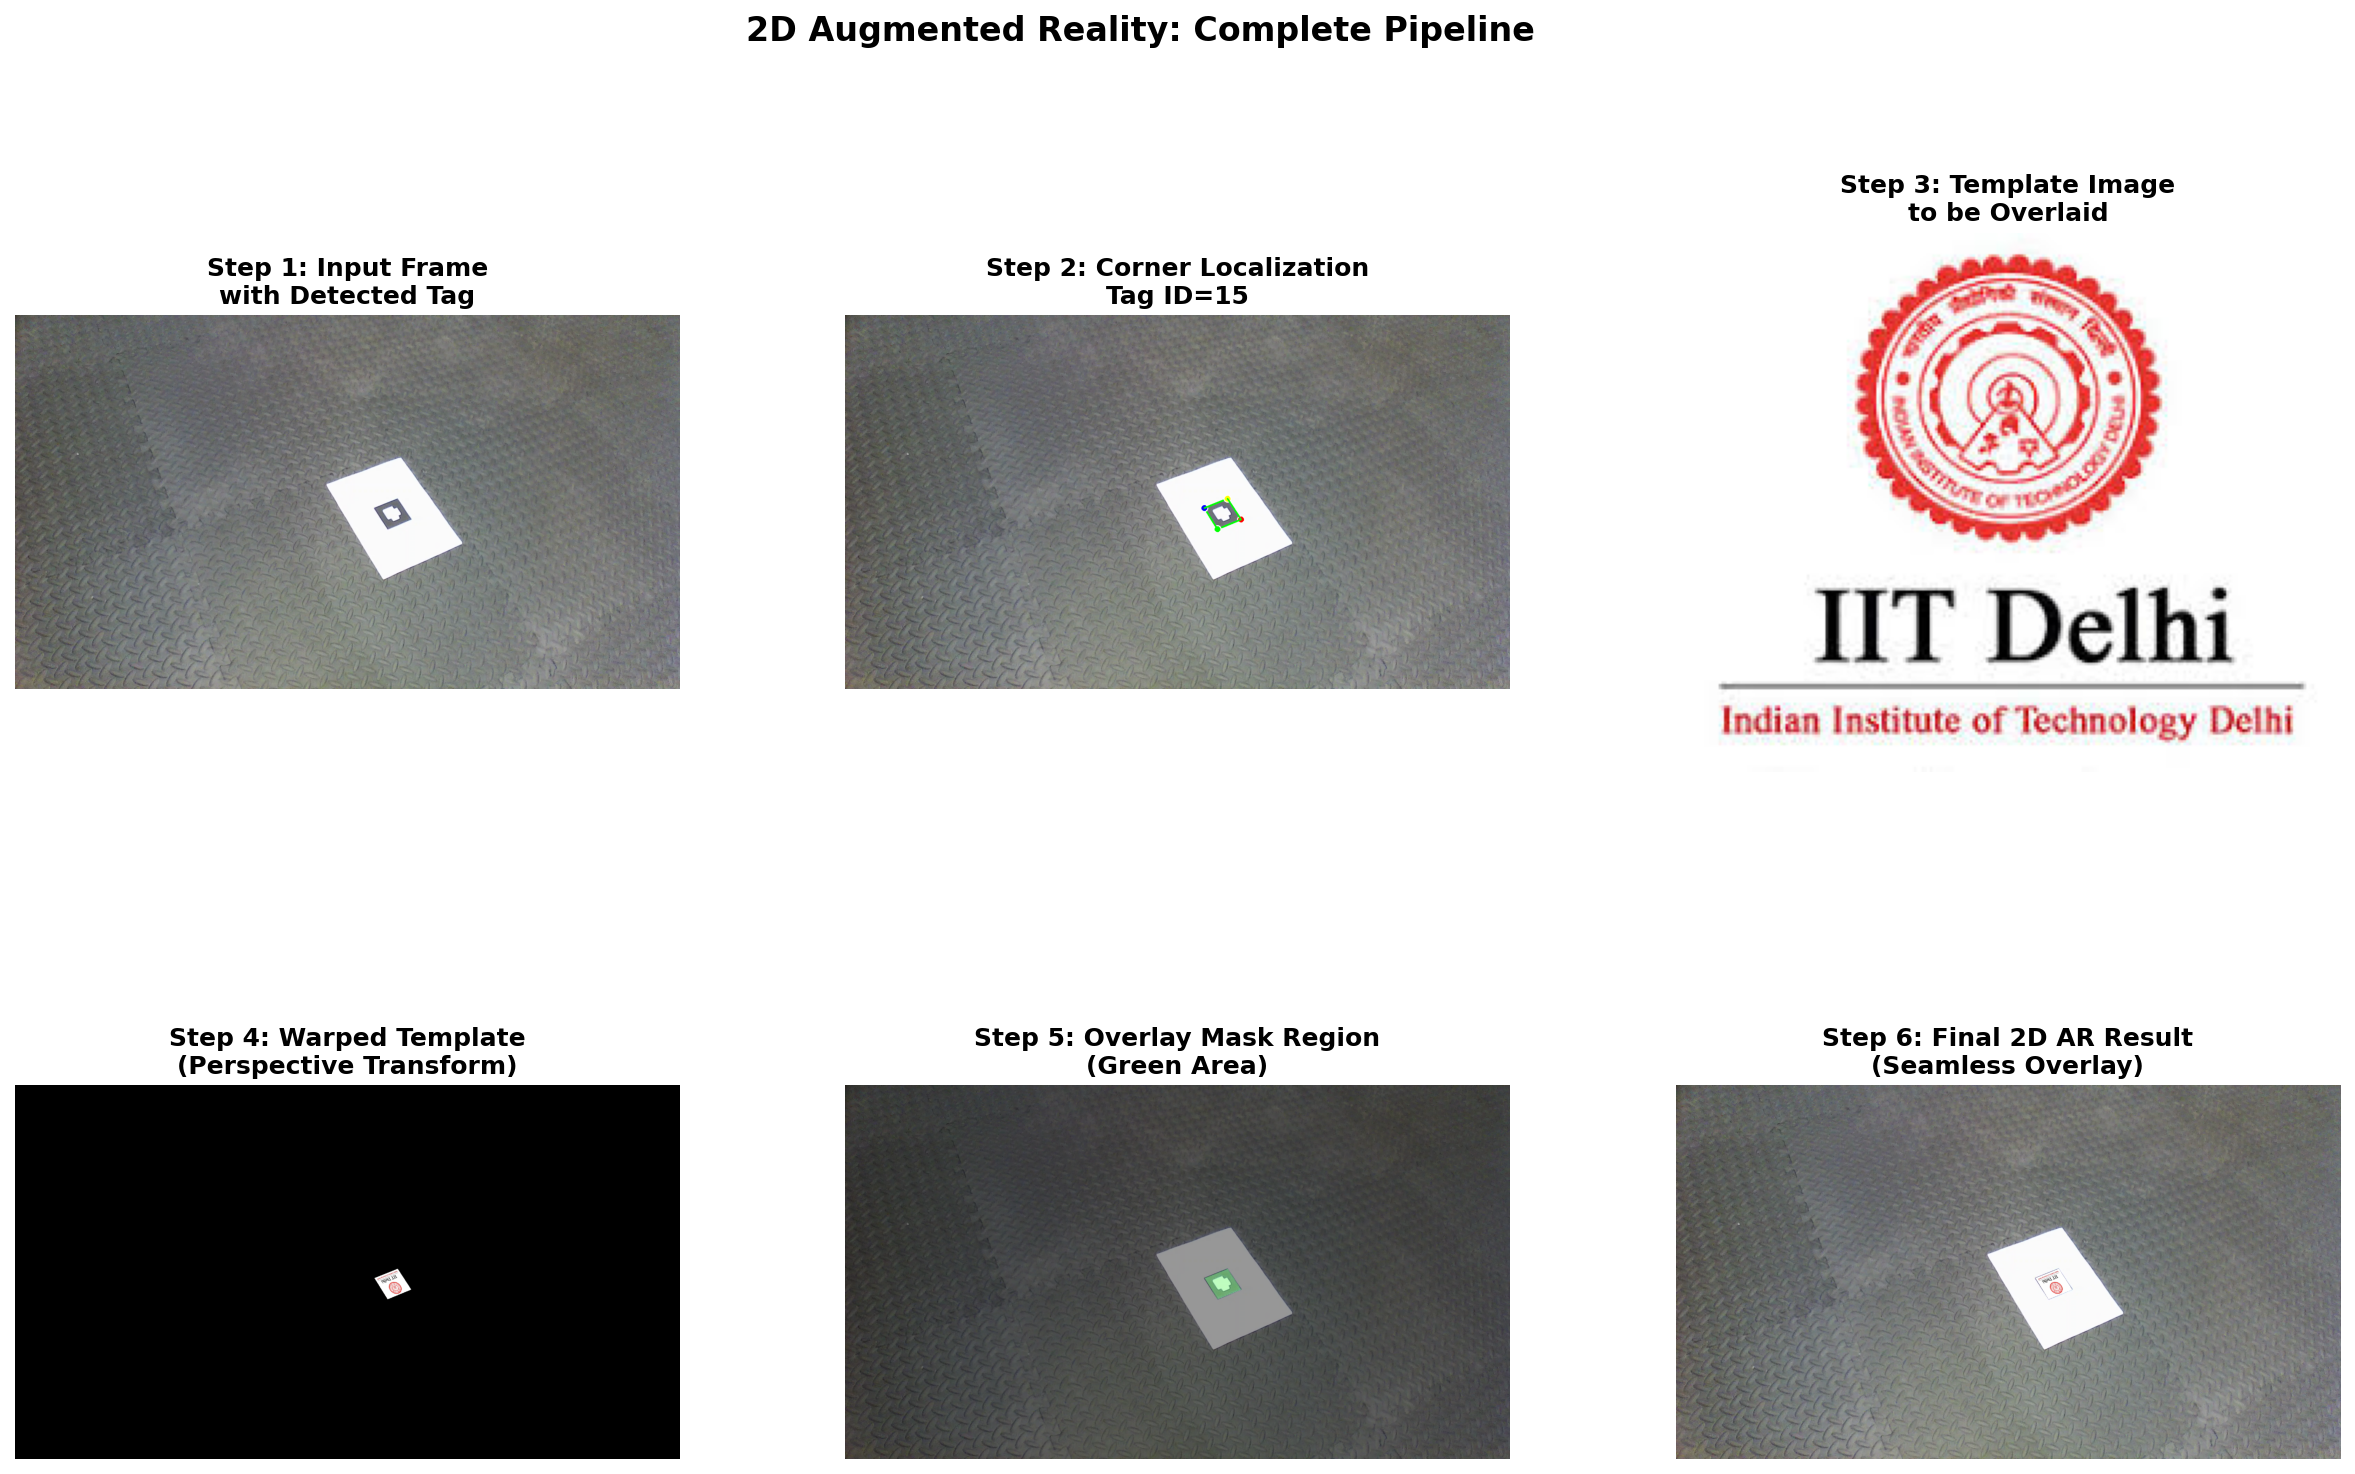
\includegraphics[width=\textwidth]{figures/2d_ar_steps.png}
        \caption{2D Augmented Reality Pipeline: (Step 1) Input frame with detected tag, (Step 2) Corner localization with color-coded vertices (red, green, blue, yellow), (Step 3) Template image to be overlaid (IITD logo), (Step 4) Warped template matching tag perspective via homography transformation, (Step 5) Overlay mask region (green area) defining blend zone, and (Step 6) Final seamless 2D AR result with template overlaid on tag.}
        \label{fig:2d_ar_steps}
    \end{figure*}


\section{3D Augmented Reality}
    video\_link - \href{https://drive.google.com/drive/folders/16X_WDvfl9n68S6WYkVBHexkdCoiUuPGZ?usp=drive_link}{click\_here}
    \newline
    Now, we try to render a 3D model over the AR tag. We have to add a functionality of projecting the object onto the image plane, which requries us to estimate the pose of the tag in 3D space.

    \subsection{Camera Calibration and Intrinsics}
    The camera intrinsic matrix $K$ encodes the camera's internal parameters:
    \begin{equation}
        K = \begin{bmatrix}
            f_x & 0 & c_x \\
            0 & f_y & c_y \\
            0 & 0 & 1
        \end{bmatrix}
    \end{equation}
    where $(f_x, f_y)$ are the focal lengths in pixels and $(c_x, c_y)$ is the principal point (optical center). These parameters are obtained through camera calibration~\cite{opencv_calibration} and loaded from the intrinsics file.

    \subsection{Pose Estimation via Homography Decomposition}

    Given detected tag corners and camera intrinsics, we estimate the 3D pose through homography decomposition. The process follows these steps:

    \textbf{Step 1: Compute Homography} — Map from canonical tag coordinates $[0,0], [200,0], [200,200], [0,200]$ to detected corners using the method from Section 2.

    \textbf{Step 2: Decompose Homography} — The homography $H$ can be decomposed to extract rotation and translation:
    \begin{equation}
        A = K^{-1} H = [\mathbf{r}_1 \quad \mathbf{r}_2 \quad \mathbf{t}]
    \end{equation}
    where $\mathbf{r}_1, \mathbf{r}_2$ are the first two columns of the rotation matrix and $\mathbf{t}$ is the translation vector.

    \textbf{Step 3: Normalization} — Compute the scale factor:
    \begin{equation}
        \lambda = \frac{\|\mathbf{r}_1\| + \|\mathbf{r}_2\|}{2}
    \end{equation}
    and normalize: $\mathbf{r}_1 = \mathbf{r}_1/\lambda$, $\mathbf{r}_2 = \mathbf{r}_2/\lambda$, $\mathbf{t} = \mathbf{t}/\lambda$.

    \textbf{Step 4: Complete Rotation Matrix} — The third rotation vector is obtained via cross product:
    \begin{equation}
        \mathbf{r}_3 = \mathbf{r}_1 \times \mathbf{r}_2
    \end{equation}

    \textbf{Step 5: Enforce Orthogonality} — The approximate rotation matrix $R_{approx} = [\mathbf{r}_1 \quad \mathbf{r}_2 \quad \mathbf{r}_3]$ may not be perfectly orthogonal. We enforce orthogonality via SVD:
    \begin{equation}
        R_{approx} = U \Sigma V^T \quad \Rightarrow \quad R = U V^T
    \end{equation}

    \subsection{Projection Matrix}

    The final 3×4 projection matrix combines intrinsics and extrinsics:
    \begin{equation}
        P = K [R \mid \mathbf{t}] = K \begin{bmatrix} \mathbf{r}_1 & \mathbf{r}_2 & \mathbf{r}_3 & \mathbf{t} \end{bmatrix}
    \end{equation}
    This matrix projects 3D points in the tag's coordinate frame to 2D image pixels:
    \begin{equation}
        \begin{bmatrix} u \\ v \\ w \end{bmatrix} = P \begin{bmatrix} X \\ Y \\ Z \\ 1 \end{bmatrix}, \quad (x, y) = \left(\frac{u}{w}, \frac{v}{w}\right)
    \end{equation}

    \subsection{3D Model Loading and Rendering}

    We support Wavefront OBJ format for 3D models. The \texttt{OBJ} class parses vertex positions and face definitions:
    \begin{itemize}
        \item \textbf{Vertices}: 3D points defining the model geometry
        \item \textbf{Faces}: Polygons (typically triangles or quads) connecting vertices
    \end{itemize}

    The rendering pipeline:
    \begin{enumerate}
        \item Scale model vertices by factor $s$ (default 50.0)
        \item Translate to center above tag: $(x, y, z) \rightarrow (x + 100, y + 100, z)$
        \item Project each face's vertices using $P$: $\mathbf{p}_{2D} = P \mathbf{p}_{3D}$
        \item Rasterize filled polygons using \texttt{cv2.fillConvexPoly}
    \end{enumerate}

    \subsection{Depth Smoothing for Stability}

    The scale factor $\lambda$ directly relates to the tag's distance from the camera. To prevent depth jitter (which causes size oscillations), we apply exponential smoothing:
    \begin{equation}
        \lambda_k = \alpha \lambda_{measured} + (1-\alpha) \lambda_{k-1}
    \end{equation}
    where $\alpha = 0.1$ controls the smoothing strength. This creates a temporal low-pass filter on depth estimates.

    \subsection{Integration with Kalman Filtering}

    The 3D AR pipeline integrates Kalman filtering from Section 2 with adjusted parameters (obtained experimentally ):
    \begin{itemize}
        \item Process noise: $\sigma_Q^2 = 0.5$ (allows more motion for 3D)
        \item Measurement noise: $\sigma_R^2 = 12.0$ (tighter tracking)
        \item Innovation threshold: $\tau = 150$ pixels
    \end{itemize}


    \subsection{Implementation Results}

The 3D AR system successfully renders complex 3D models on detected AR tags at approximately 12 FPS. The approach (Kalman + depth filtering) eliminates both position jitter and scale oscillations, but still, some jitter remains due to ineffective corner detection.

    \figref{fig:3d_ar_steps} presents the complete 3D AR rendering pipeline. The process begins with camera calibration and pose estimation, visualizes the 3D coordinate frame, shows wireframe projection, and concludes with solid model rendering.

    \begin{figure*}[t]
        \centering
        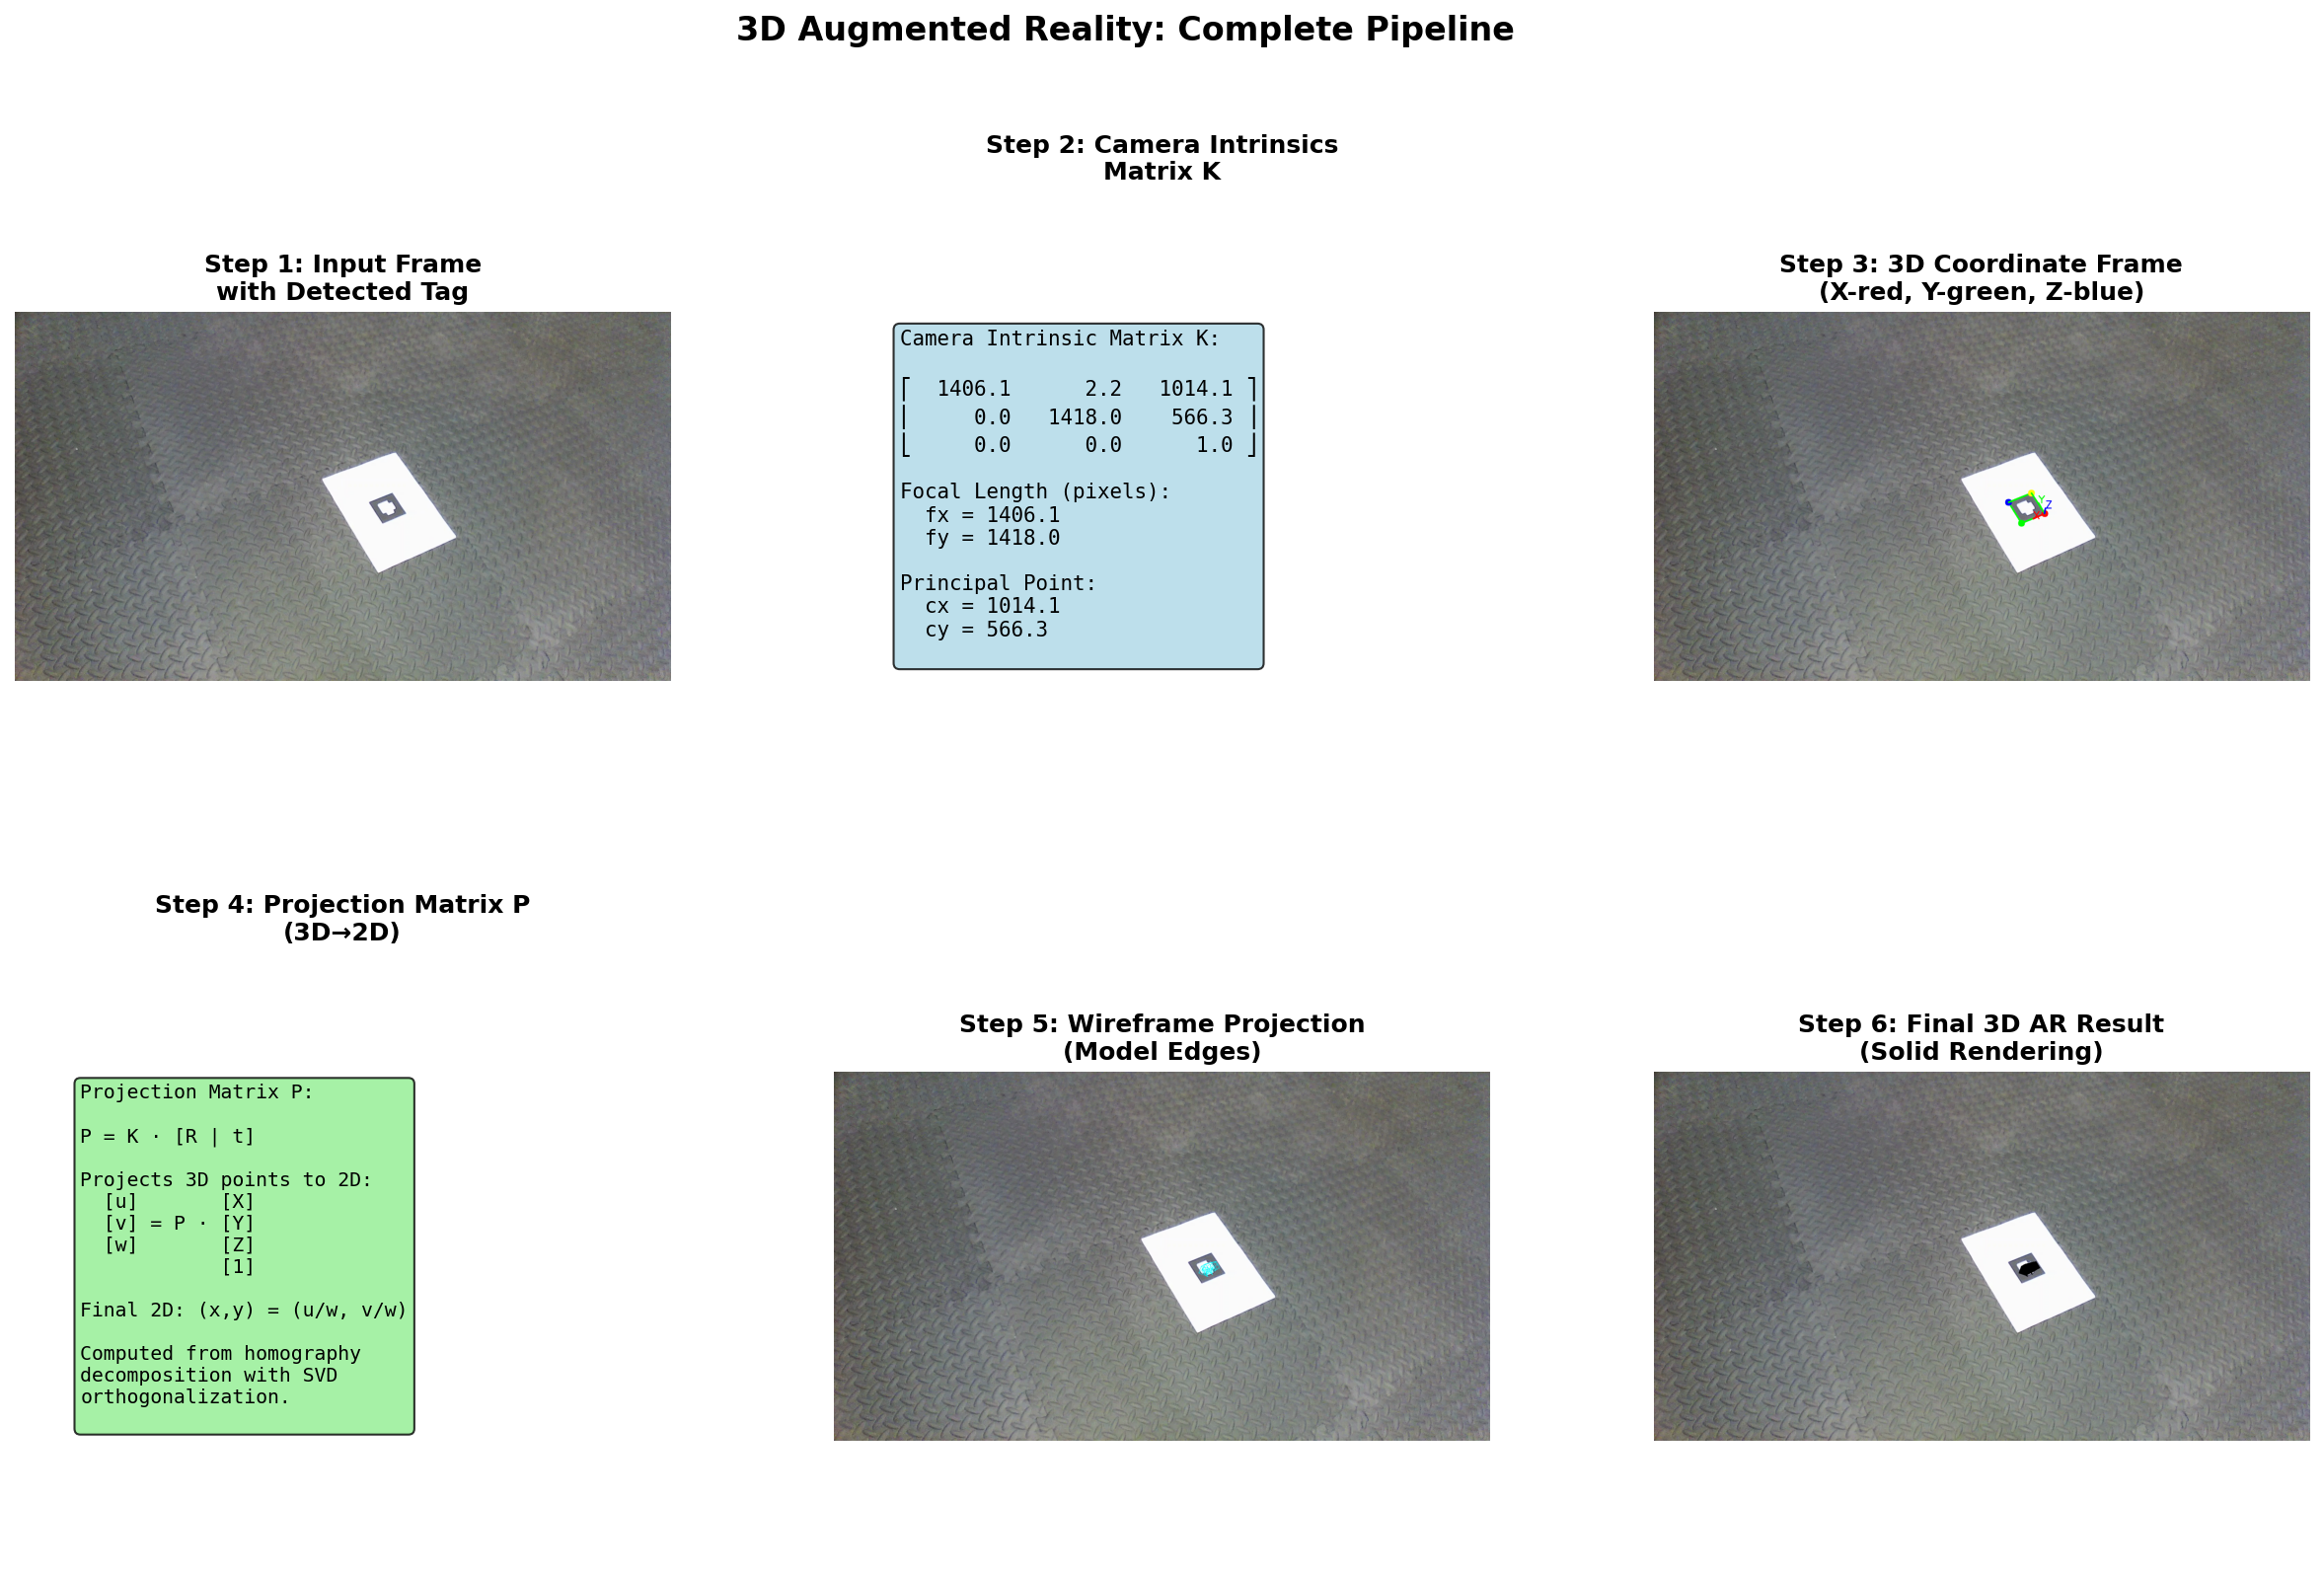
\includegraphics[width=\textwidth]{figures/3d_ar_steps.png}
        \caption{3D Augmented Reality Pipeline: (Step 1) Input frame with detected tag, (Step 2) Camera intrinsic matrix K showing focal lengths (fx=1406.1, fy=1418.0) and principal point, (Step 3) 3D coordinate frame visualization with X-axis (red), Y-axis (green), and Z-axis (blue) projected onto the tag, (Step 4) Projection matrix P computed via homography decomposition with SVD orthogonalization, (Step 5) Wireframe projection showing 3D model edges mapped to 2D image plane, and (Step 6) Final solid 3D rendering with face rasterization.}
        \label{fig:3d_ar_steps}
    \end{figure*}


\section{Critiques on model Performance:}
\begin{itemize}
    \item The detection pipeline is able to detect AR tags with an average FPS of around 12, but it is very sensitive to the movement of the camera. If the camera is moving too fast, the detection fails to keep track, but as the camera stabilizes, the detection is able to catch up.
    \item The detection pipeline is heavilty dependent on background. If the background is bright enough, the thresholding step fails to segeragate the A4 sheets from the background. We have also used Otsu's thresholding method, but it did not work well for our images, as it was not able to accurately segment the A4 sheets from the background, if it was too bright, as can be seen in some videos of webcamera.
    \item The detection pipeline still shows some jitter, some of it might be reduced by optimising the parameters of the Kalman filter, but the main source of jitter is the noise in the detected corners, due to blurriness. 
\end{itemize}


\appendix

\section{Kalman Filter for Corner Tracking}

    This appendix provides the detailed mathematical formulation of the Kalman filter used for temporal smoothing of AR tag corners in the 2D augmented reality pipeline.
    \newline
    \subsection{State Space Model}

    Each corner is tracked independently using a constant velocity motion model. The state vector at time $k$ is:
    \begin{equation}
        \mathbf{x}_k = \begin{bmatrix} x_k \\ y_k \\ v_{x,k} \\ v_{y,k} \end{bmatrix}
    \end{equation}
    where $(x_k, y_k)$ represents the corner position in pixels and $(v_{x,k}, v_{y,k})$ represents the velocity in pixels per frame.

    \subsection{State Transition Model}

    The discrete-time state transition follows a linear dynamical system:
    \begin{equation}
        \mathbf{x}_{k+1} = F \mathbf{x}_k + \mathbf{w}_k
    \end{equation}
    where $F$ is the state transition matrix and $\mathbf{w}_k \sim \mathcal{N}(0, Q)$ is the process noise.

    The state transition matrix for constant velocity motion with time step $\Delta t = 1$ frame is:
    \begin{equation}
        F = \begin{bmatrix}
            1 & 0 & \Delta t & 0 \\
            0 & 1 & 0 & \Delta t \\
            0 & 0 & 1 & 0 \\
            0 & 0 & 0 & 1
        \end{bmatrix}
    \end{equation}

    This model assumes that position evolves according to current velocity: $x_{k+1} = x_k + v_{x,k} \cdot \Delta t$, and velocity remains constant: $v_{x,k+1} = v_{x,k}$.

    \subsection{Measurement Model}

    The measurement model relates the observed corner positions to the state:
    \begin{equation}
        \mathbf{z}_k = H \mathbf{x}_k + \mathbf{v}_k
    \end{equation}
    where $\mathbf{z}_k = [z_{x,k}, z_{y,k}]^T$ are the detected corner coordinates, $H$ is the measurement matrix, and $\mathbf{v}_k \sim \mathcal{N}(0, R)$ is the measurement noise.

    Since we only observe position (not velocity), the measurement matrix is:
    \begin{equation}
        H = \begin{bmatrix}
            1 & 0 & 0 & 0 \\
            0 & 1 & 0 & 0
        \end{bmatrix}
    \end{equation}

    \subsection{Kalman Filter Recursion}

    The Kalman filter operates in two phases:

    \textbf{Prediction Step:}
    \begin{align}
        \hat{\mathbf{x}}_{k|k-1} &= F \hat{\mathbf{x}}_{k-1|k-1} \\
        P_{k|k-1} &= F P_{k-1|k-1} F^T + Q
    \end{align}
    where $\hat{\mathbf{x}}_{k|k-1}$ is the predicted state and $P_{k|k-1}$ is the predicted error covariance.

    \textbf{Update Step:}
    \begin{align}
        \mathbf{y}_k &= \mathbf{z}_k - H \hat{\mathbf{x}}_{k|k-1} \quad \text{(Innovation)} \\
        S_k &= H P_{k|k-1} H^T + R \quad \text{(Innovation covariance)} \\
        K_k &= P_{k|k-1} H^T S_k^{-1} \quad \text{(Kalman gain)} \\
        \hat{\mathbf{x}}_{k|k} &= \hat{\mathbf{x}}_{k|k-1} + K_k \mathbf{y}_k \\
        P_{k|k} &= (I - K_k H) P_{k|k-1}
    \end{align}

    \subsection{Noise Covariance Matrices}

    The \textbf{process noise covariance} $Q$ models uncertainty in the motion model:
    \begin{equation}
        Q = \begin{bmatrix}
            \sigma_Q^2 & 0 & 0 & 0 \\
            0 & \sigma_Q^2 & 0 & 0 \\
            0 & 0 & 2\sigma_Q^2 & 0 \\
            0 & 0 & 0 & 2\sigma_Q^2
        \end{bmatrix}
    \end{equation}
    We use $\sigma_Q^2 = 0.2$ for 2D overlay, with higher uncertainty in velocity components.

    The \textbf{measurement noise covariance} $R$ models detection uncertainty:
    \begin{equation}
        R = \begin{bmatrix}
            \sigma_R^2 & 0 \\
            0 & \sigma_R^2
        \end{bmatrix}
    \end{equation}
    We use $\sigma_R^2 = 30.0$ to account for pixel-level corner detection jitter.

    \subsection{Outlier Rejection}

    To handle occlusions and detection failures, we implement innovation-based outlier rejection. The innovation is:
    \begin{equation}
        \text{Innovation} = \|\mathbf{y}_k\| = \|\mathbf{z}_k - H \hat{\mathbf{x}}_{k|k-1}\|
    \end{equation}

    If the innovation exceeds threshold $\tau_{innov} = 150$ pixels, we reject the measurement and reinitialize the filter:
    \begin{equation}
        \text{if } \|\mathbf{y}_k\| > \tau_{innov} \text{ then reinitialize with } \hat{\mathbf{x}}_{k|k} = [z_{x,k}, z_{y,k}, 0, 0]^T
    \end{equation}

    \subsection{Rigid Quadrilateral Constraint}

    After independently filtering all four corners, we enforce geometric consistency by reconstructing the fourth corner as:
    \begin{equation}
        \mathbf{c}_2 = \mathbf{c}_0 + (\mathbf{c}_1 - \mathbf{c}_0) + (\mathbf{c}_3 - \mathbf{c}_0)
    \end{equation}
    where $\mathbf{c}_i = [x_i, y_i]^T$ are the filtered corner positions. This ensures the quadrilateral forms a parallelogram, preventing distortions from drift between independent filters.

\section{Flood-Fill Algorithm for ROI Separation}

    The flood-fill algorithm (also known as seed-fill or boundary-fill) is used in Step 2 of the detection pipeline to identify connected white regions (A4 sheets) in the thresholded binary image. We use a Breadth-First Search (BFS) approach on a downsampled image for efficiency.

    \subsection{Algorithm Overview}

    Given a binary image $B \in \{0, 255\}^{h \times w}$ and downsampling factor $s=8$, we first create a downsampled version:
    \begin{equation}
        B_{small}[i, j] = B[i \cdot s, j \cdot s] \quad \forall i \in [0, h/s), j \in [0, w/s)
    \end{equation}

    \subsection{BFS-Based Connected Component Detection}

    For each unvisited white pixel $(y_0, x_0)$ in $B_{small}$, we perform BFS to find all connected white pixels:

    \begin{enumerate}
        \item Initialize queue $Q \leftarrow \{(y_0, x_0)\}$ and visited set $V \leftarrow \emptyset$
        \item Mark $(y_0, x_0)$ as visited: $V \leftarrow V \cup \{(y_0, x_0)\}$
        \item While $Q \neq \emptyset$:
        \begin{itemize}
            \item Dequeue $(y, x) \leftarrow Q$
            \item Add $(y \cdot s, x \cdot s)$ to current island (scaled back to original coordinates)
            \item For each 4-connected neighbor $(y', x') \in \{(y-1,x), (y+1,x), (y,x-1), (y,x+1)\}$:
            \begin{itemize}
                \item If $B_{small}[y', x'] = 255$ and $(y', x') \notin V$:
                \item Mark visited: $V \leftarrow V \cup \{(y', x')\}$
                \item Enqueue: $Q \leftarrow Q \cup \{(y', x')\}$
            \end{itemize}
        \end{itemize}
        \item Return island if size $\geq$ minimum area threshold
    \end{enumerate}

    \subsection{Complexity Analysis}

    Let $n = h \times w$ be the total number of pixels.
    \begin{itemize}
        \item \textbf{Without downsampling}: $O(n)$ time, $O(n)$ space for visited array
        \item \textbf{With downsampling by $s$}: $O(n/s^2)$ time for BFS, reducing from $O(1920 \times 1080) = O(2M)$ to $O(240 \times 135) = O(32K)$ for our 1080p images with $s=8$
        \item The ROI expansion step (iterative boundary checking) adds $O(s \cdot p)$ where $p$ is the perimeter of the island
    \end{itemize}

    This downsampling approach provides a $64\times$ speedup while maintaining detection accuracy since A4 sheets span many pixels.

\section{Fast Component Labeling with Stack-Based DFS}

    Fast component labeling (Step 3) identifies the largest black connected component within each ROI that doesn't touch the border. This component represents the AR tag marker. We use an iterative depth-first search (DFS) with explicit stack to avoid recursion limits.

    \subsection{Algorithm}

    Given ROI binary image $R \in \{0, 255\}^{h_{roi} \times w_{roi}}$:

    \begin{enumerate}
        \item Initialize $visited \in \{0, 1\}^{h_{roi} \times w_{roi}} \leftarrow 0$, $max\_area \leftarrow 0$
        \item For each pixel $(y, x) \in R$:
        \begin{itemize}
            \item If $R[y, x] = 0$ (black) and not visited:
            \begin{enumerate}
                \item Initialize stack $S \leftarrow \{(y, x)\}$, component $C \leftarrow \emptyset$
                \item Set $visited[y, x] \leftarrow 1$, $touches\_border \leftarrow \text{False}$
                \item While $S \neq \emptyset$:
                \begin{itemize}
                    \item Pop $(y_c, x_c) \leftarrow S$
                    \item Add $(y_c, x_c)$ to $C$
                    \item If $(y_c, x_c)$ is on border: $touches\_border \leftarrow \text{True}$
                    \item For each 4-neighbor $(y_n, x_n)$:
                    \begin{itemize}
                        \item If $R[y_n, x_n] = 0$ and not visited:
                        \item Mark visited: $visited[y_n, x_n] \leftarrow 1$
                        \item Push: $S \leftarrow S \cup \{(y_n, x_n)\}$
                    \end{itemize}
                \end{itemize}
                \item If $\neg touches\_border$ and $|C| > max\_area$:
                \begin{itemize}
                    \item Update: $max\_area \leftarrow |C|$, $best\_component \leftarrow C$
                \end{itemize}
            \end{enumerate}
        \end{itemize}
        \item Return boundary pixels of $best\_component$ (via erosion)
    \end{enumerate}

    \subsection{Boundary Extraction via Erosion}

    To extract boundary pixels efficiently:
    \begin{align}
        boundary[y, x] = mask[y, x] \land \neg (&mask[y-1, x] \land \nonumber\\
        &mask[y+1, x] \land \nonumber\\
        &mask[y, x-1] \land \nonumber\\
        &mask[y, x+1])
    \end{align}
    where $mask$ is a binary indicator of pixels in $best\_component$. This morphological operation identifies pixels adjacent to at least one background pixel.

    \subsection{Complexity}

    Each pixel is visited at most once: $O(h_{roi} \times w_{roi})$. For typical ROIs of $300 \times 300$, this is $O(90K)$ operations, which is manageable even without further optimization.

\section{Convex Hull: Andrew's Monotone Chain Algorithm}

    The convex hull (Step 4) finds the minimal convex polygon containing all boundary points. We implement Andrew's monotone chain algorithm, which is simpler and more numerically stable than Graham scan.

    \subsection{Algorithm}

    Given $n$ points $P = \{(x_i, y_i)\}_{i=1}^n$:

    \textbf{Step 1: Sort Points}
    \begin{equation}
        P_{sorted} = \text{sort}(P, \text{key}=(x, y)) \quad \text{(lexicographic order)}
    \end{equation}

    \textbf{Step 2: Build Lower Hull}
    \begin{enumerate}
        \item Initialize $L \leftarrow []$
        \item For $i = 0$ to $n-1$:
        \begin{itemize}
            \item While $|L| \geq 2$ and $\text{cross}(L[-2], L[-1], P_i) \leq 0$:
            \begin{itemize}
                \item Pop $L[-1]$ (remove non-left turn)
            \end{itemize}
            \item Append $P_i$ to $L$
        \end{itemize}
    \end{enumerate}

    \textbf{Step 3: Build Upper Hull}
    \begin{enumerate}
        \item Initialize $U \leftarrow []$
        \item For $i = n-1$ down to $0$:
        \begin{itemize}
            \item While $|U| \geq 2$ and $\text{cross}(U[-2], U[-1], P_i) \leq 0$:
            \begin{itemize}
                \item Pop $U[-1]$
            \end{itemize}
            \item Append $P_i$ to $U$
        \end{itemize}
    \end{enumerate}

    \textbf{Step 4: Concatenate}
    \begin{equation}
        \text{ConvexHull}(P) = L[:-1] \oplus U[:-1]
    \end{equation}
    (Remove last point from each hull to avoid duplication of endpoints)

    \subsection{Cross Product Test}

    The cross product determines turn direction:
    \begin{equation}
        \text{cross}(A, B, C) = (B_x - A_x)(C_y - B_y) - (B_y - A_y)(C_x - B_x)
    \end{equation}
    \begin{itemize}
        \item $\text{cross} > 0$: Left turn (counter-clockwise)
        \item $\text{cross} < 0$: Right turn (clockwise)
        \item $\text{cross} = 0$: Collinear
    \end{itemize}

    For the lower hull, we keep only left turns (reject right turns and collinear points). For the upper hull, the reverse traversal ensures the same criterion applies.

    \subsection{Complexity}

    \begin{itemize}
        \item Sorting: $O(n \log n)$
        \item Hull construction: $O(n)$ (each point pushed/popped at most once)
        \item Total: $O(n \log n)$
    \end{itemize}

    For typical AR tag boundaries with $n \approx 200$-$500$ pixels, this is very efficient.

\section{Douglas-Peucker Polygon Approximation}

    The Douglas-Peucker algorithm (also called Ramer-Douglas-Peucker) simplifies a polygon by recursively removing points whose distance from the approximating line segment is below a threshold $\epsilon$. This is crucial for extracting exactly 4 corners from the convex hull in Step 4.

    \subsection{Recursive Algorithm}

    Given polyline $P = [p_0, p_1, \ldots, p_n]$ and tolerance $\epsilon$:

    \begin{enumerate}
        \item Draw line segment $\overline{p_0 p_n}$ connecting first and last points
        \item Find point $p_k$ with maximum perpendicular distance $d_{max}$ from $\overline{p_0 p_n}$:
        \begin{equation}
            k = \arg\max_{i \in [1, n-1]} d(p_i, \overline{p_0 p_n})
        \end{equation}
        \item If $d_{max} > \epsilon$:
        \begin{itemize}
            \item Recursively simplify $P[0:k+1]$ (left segment)
            \item Recursively simplify $P[k:n+1]$ (right segment)
            \item Concatenate results (removing duplicate $p_k$)
        \end{itemize}
        \item Else:
        \begin{itemize}
            \item Return $[p_0, p_n]$ (discard all intermediate points)
        \end{itemize}
    \end{enumerate}

    \subsection{Point-to-Line Distance}

    For point $P$ and line through $A$ and $B$, the perpendicular distance is:
    \begin{equation}
        d(P, \overline{AB}) = \frac{|(B_x - A_x)(A_y - P_y) - (A_x - P_x)(B_y - A_y)|}{\sqrt{(B_x - A_x)^2 + (B_y - A_y)^2}}
    \end{equation}

    However, for numerical efficiency, we can work with squared distances (avoiding square root) until the final comparison:
    \begin{equation}
        \text{Let } \mathbf{v} = B - A, \quad t = \frac{(P - A) \cdot \mathbf{v}}{\|\mathbf{v}\|^2}
    \end{equation}
    \begin{equation}
        \text{Projection: } P_{proj} = A + t \mathbf{v}, \quad d = \|P - P_{proj}\|
    \end{equation}

    \subsection{Adaptive Epsilon Selection}

    For AR tag corner detection, we use adaptive $\epsilon$ based on perimeter:
    \begin{equation}
        \epsilon = \alpha \cdot \text{perimeter}(\text{ConvexHull}), \quad \alpha \in [0.01, 0.08]
    \end{equation}

    We iteratively try increasing $\alpha$ values until exactly 4 corners are obtained. This handles varying tag sizes and perspectives robustly.

    \subsection{Complexity}

    \begin{itemize}
        \item Worst case: $O(n^2)$ (e.g., semi-circle approximation)
        \item Best/average case: $O(n \log n)$ (balanced recursion tree)
        \item For convex hulls with $n \approx 100$ points, typically produces result in $<10$ iterations
    \end{itemize}

\section{Homography Computation via SVD}

    Computing the homography matrix $H$ that maps source points to destination points is fundamental to both tag decoding (Step 5) and 2D overlay (Section 2). We solve this using Singular Value Decomposition (SVD) of the Direct Linear Transform (DLT) formulation. The implementation follows the approach described in~\cite{rastogi_artag}.

    \subsection{Homogeneous Coordinates}

    A homography maps points in projective space:
    \begin{equation}
        \begin{bmatrix} u' \\ v' \\ w' \end{bmatrix} = H \begin{bmatrix} u \\ v \\ 1 \end{bmatrix}, \quad (x', y') = \left(\frac{u'}{w'}, \frac{v'}{w'}\right)
    \end{equation}
    where $H \in \mathbb{R}^{3 \times 3}$ has 8 degrees of freedom (9 parameters up to scale).

    \subsection{Direct Linear Transform (DLT)}

    Given 4 point correspondences $\{(x_i, y_i) \leftrightarrow (x'_i, y'_i)\}_{i=1}^4$, we construct the constraint matrix $A \in \mathbb{R}^{8 \times 9}$:
    \begin{equation}
        A = \begin{bmatrix}
            -x_1 & -y_1 & -1 & 0 & 0 & 0 & x'_1 x_1 & x'_1 y_1 & x'_1 \\
            0 & 0 & 0 & -x_1 & -y_1 & -1 & y'_1 x_1 & y'_1 y_1 & y'_1 \\
            -x_2 & -y_2 & -1 & 0 & 0 & 0 & x'_2 x_2 & x'_2 y_2 & x'_2 \\
            0 & 0 & 0 & -x_2 & -y_2 & -1 & y'_2 x_2 & y'_2 y_2 & y'_2 \\
            \vdots & \vdots & \vdots & \vdots & \vdots & \vdots & \vdots & \vdots & \vdots
        \end{bmatrix}
    \end{equation}

    Each point correspondence provides 2 linear equations (one for $x'$, one for $y'$). Four points give 8 equations for 8 unknowns (the 9th parameter is fixed by normalization).

    \subsection{SVD Solution}

    We seek $\mathbf{h} = [h_{11}, h_{12}, h_{13}, h_{21}, h_{22}, h_{23}, h_{31}, h_{32}, h_{33}]^T$ that minimizes $\|A\mathbf{h}\|$ subject to $\|\mathbf{h}\| = 1$.

    \textbf{Step 1: Compute SVD}
    \begin{equation}
        A = U \Sigma V^T
    \end{equation}

    \textbf{Step 2: Extract Solution}
    The solution is the last column of $V$ (corresponding to smallest singular value):
    \begin{equation}
        \mathbf{h} = V[:, -1]
    \end{equation}

    \textbf{Step 3: Normalize and Reshape}
    \begin{equation}
        \mathbf{h} \leftarrow \frac{\mathbf{h}}{\mathbf{h}[8]}, \quad H = \text{reshape}(\mathbf{h}, 3 \times 3)
    \end{equation}
    This ensures $H[2, 2] = 1$ (standard normalization).

    \subsection{Numerical Stability}

    SVD is numerically stable and handles:
    \begin{itemize}
        \item Nearly degenerate configurations (coplanar or collinear points)
        \item Noise in point correspondences
        \item Overdetermined systems (more than 4 point pairs)
    \end{itemize}

    The condition number $\kappa(A) = \sigma_{max} / \sigma_{min}$ indicates solution quality. For well-conditioned problems (AR tags viewed nearly fronto-parallel), $\kappa(A) < 100$.

    \subsection{Complexity}

    SVD via Golub-Reinsch algorithm: $O(mn^2)$ for $A \in \mathbb{R}^{m \times n}$. For our case with $m=8$, $n=9$: $O(8 \times 9^2) = O(648)$ operations, effectively constant time.

%----------------------------------------------------------

\section*{Acknowledgments}
The implementation of homography computation and AR tag detection pipeline was influenced by the work in~\cite{rastogi_artag}. Camera calibration techniques follow the methods described in~\cite{opencv_calibration}. Kalman filter implementation was guided by~\cite{rlabbe_kalman}. Perspective warping utilizes OpenCV functions~\cite{opencv_warp}. Performance optimization was enabled by the Numba JIT compiler~\cite{numba_jit}.

\section*{Code Repository}
The complete source code for this project is available at: \href{https://github.com/shahi-dKhan/col780-AR_tags_analysus}{https://github.com/shahi-dKhan/col780-AR\_tags\_analysus}

%----------------------------------------------------------

\printbibliography[heading=bibintoc,title={References}]

%----------------------------------------------------------

\end{document}